\chapter[Search for top squarks in all-hadronic final states]{Search for top squarks in all-hadronic final states}
\label{ch:stop_ana}
\epigraph{\emph{In God we trust. All others must bring data.}}{William E. Deming}

	In this chapter the core of this thesis will be presented, namely the search for the direct pair-production of the supersymmetric partner of the top quark in all-hadronic final states using a dataset of $36.1\, \ifb$ \pp\ collisions, at a centre-of-mass energy $\rts = 13$ \TeV, delivered by the \ac{LHC} and collected by the \ac{ATLAS} detector. %A dataset of $36.1\, \ifb$ was used. Such measured value of integrated luminosity has an uncertainty of 3.2\% based on studies of scans of the $x-y$ beam separation carried out on both $2015$ and $2016$ datasets, where the average pileup parameter $\mu$ was $13.7$ and $24.9$, respectively.
		
	The results produced were published in a paper in the Journal of High Energy Physics in September 2017~\cite{stop0L}. A previous version of the analysis was also made public, using $13.3\,\ifb$ collected at $\rts = 13$ \TeV, with an earlier subset of the whole $2015+2016$ dataset, documented in an ATLAS conference note~\cite{ICHEPstop0L}. Although both versions contain author's contributions, only the results of the most recent analysis will be hereby discussed, as it represents the most updated, improved and extended version. Specifically, the optimisation of the search strategy, as well as the data-driven estimation of the number of events in the search regions for one of the most important backgrounds, and the evaluation of the related theory uncertainties, characterised the author's contributions. In addition, exception made for the optimisation strategy, the same contributions were also used in a different \ac{SUSY} analysis published in October 2017 in~\cite{DMhf}. Further details can be found in Appendix~\ref{ch:appA}.

	The chapter will be structured as it follows: an excursus on the simplified \ac{SUSY} models considered will be presented in Section~\ref{sec:susysig}; the objects used in both data and \ac{MC} will be discussed in Section~\ref{sec:obj_def}; the selection of the events, together with the key variables used and the optimisation of the regions in which the \ac{SUSY} signals were searched for will be presented in in Section~\ref{sec:evtsel}; the nominal procedure used for the background estimation will be discussed in Section~\ref{sec:bkgest}, with particular focus on the data-driven background estimation in Section~\ref{sec:ddbkgest}; the results, together with their interpretation, will finally be presented in Section~\ref{sec:results}.


	\section{SUSY Signals}
	\label{sec:susysig}

		As already introduced in Section~\ref{sec:SUSYPheno}, the signals considered in this work are generated using simplified models, meaning that only the \stop, the \ninoone, the \ninotwo, and the \chinoonepm, were the \ac{SUSY} particles considered. In particular, in such considered models, either \ninotwo\ or \chinoonepm\ is assumed to be the \ac{NLSP} and, the chargino-neutralino mass splitting $\Delta m(\chinoonepm, \ninoone)$ is assumed to be $1$ \GeV, in accordance with the naturalness argument. This implies that the \chinoonepm\ will promptly decay to $\Wboson^*\ninoone$ , with the \Wboson\ emitted as a virtual particle. The decay products of the so-created virtual \Wboson\ will therefore be low \pt\ objects which will not be reconstructed by the \ac{ATLAS} detector. 

		\subsection{Benchmark processes}

			\begin{figure}[!htb]
				% \begin{center}
				\centering
					\subbottom[$\stop\ra t^{(*)}\ninoone$]{
						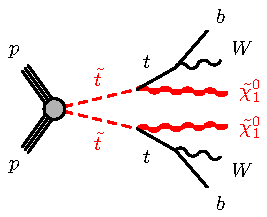
\includegraphics[width=0.28\textwidth]{theory/stst-bqqbqqN1N1-tt}}\hspace{0.05\textwidth}
					\subbottom[$\stop\ra b\ \chinoonepm\ra b \Wboson^{(*)}\ninoone$]{
						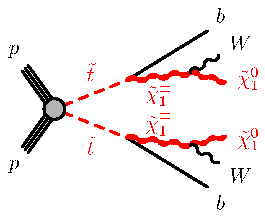
\includegraphics[width=0.28\textwidth]{theory/stst-bbWWN1N1}}\hspace{0.05\textwidth}
					\subbottom[$\stop\ra t\ \ninotwo\to h/Z\ \ninoone$]{
						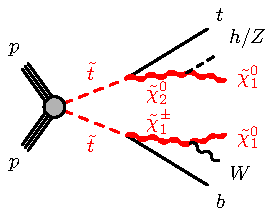
\includegraphics[width=0.28\textwidth]{theory/stst-tbhWN1N1}}\hspace{0.05\textwidth}
				% \end{center}
				\caption{Diagrams of the decay topologies of the signal models considered in this work.}
				\label{fig:stopModels}
			\end{figure}

			Figure~\ref{fig:stopModels}(a)$-$(c) shows the diagrams corresponding to the decay scenarios considered in this work. In particular, (a) where both top squarks decay\footnote{The symbol (*) indicates off-shell production} via $\stop\rightarrow t^{(*)}\ \ninoone$; (b) where at least one of the stops decays via $\stop\rightarrow b\ \chinoonepm \rightarrow b\ \Wboson^{(*)}\ \ninoone$; (c) where $m_{\ninotwo}$ is small enough to allow one stop to decay via $\stop\to t\ \ninotwo \to h/Z\ \ninoone$ where $h$ is the \ac{SM} Higgs boson;

			\begin{wrapfigure}{R}{.5\textwidth}
				\centering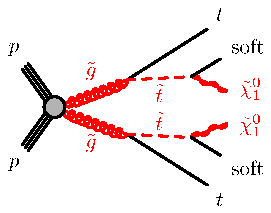
\includegraphics[width=.28\textwidth]{theory/gogo-tsofttsoftN1N1-stst}
				\caption{Diagram of the gluino-mediated top squark production. The term ``soft" refers to decay products whose transverse momenta are below the detector thresholds.}
				\label{fig:gtt}
			\end{wrapfigure}

			The results were interpreted in the simplified models where only one- and two-step decays scenarios are allowed and, as already mentioned, the latter will be referred to as a natural \ac{SUSY}-inspired mixed grid, \ie\ $\Delta m(\chinoonepm, \ninoone) = 1 \GeV$~\cite{Alwall:2008ve, Alwall:2008ag, Alves:2011wf}. Furthermore, in both scenarios the \ac{LSP} is considered to be a pure bino state. The results will also be interpreted in two slices of the \ac{pMSSM} models: wino-\ac{NLSP} and well-tempered neutralino \ac{pMSSM}~\cite{Djouadi:1998di, Berger:2008cq}.
			A fourth scenario, in addition to direct pair production, was considered: top squarks can also be indirectly produced via gluino decays, as illustrated in Figure~\ref{fig:gtt}. In such model, the mass difference between the top squark and the neutralino is considered to be relatively small, $\Delta m(\stopone, \ninoone) = 5$ \GeV, allowing the jets originating from \stopone\ decay to have a \pt\ below the reconstruction threshold of the \ac{ATLAS} detector resulting in an experimental signature nearly equivalent to the one in Figure~\ref{fig:stopModels}(a).


		\subsection{MC samples}

			A grid of points across the $(\mstopone-\mninoone)$ plane with a $50$-\GeV\ spacing is generated to simulate the above-mentioned simplified models. %The mixing between the partners of the left- and right-handed top quarks is assumed to be maximal, \ie\ ..
			The signal models were generated using \texttt{MG5\_aMC@NLO 2.2-2.4}~\cite{madgraph} interfaced to \texttt{PYTHIA8}~\cite{pythia8} for the \ac{PS} and hadronisation. \texttt{EvtGen 1.2.0}~\cite{evtGen} was employed for the decays of the  $b$- and $c$-hadrons. The tree-level \ac{ME} calculation includes the emission of up to two additional partons for all signal samples. The \texttt{NNPDF2.3LO} \ac{PDF}~\cite{PDFs} set was used to generate the signal samples with the \texttt{A14}~\cite{CT10} tune for the \ac{UE} and shower parameters. Additionally, the CKKW-L prescription~\cite{CKKW} was used for the \ac{ME}–\ac{PS} matching. 

			The various signal cross sections were all calculated to next-to-leading order in the strong coupling constant, with the addition of soft-gluon emission re-summation at next-to-leading-logarithm accuracy (NLO+NLL)~\cite{Beenakker:1997ut, Beenakker:2010nq, Beenakker:2011fu}. The sparticle mass spectra for \ac{pMSSM} models were calculated using \texttt{Softsusy 3.7.3}~\cite{Allanach:2001kg, Allanach:2013kza} while the decays of each sparticle were performed by \texttt{HDECAY 3.4}~\cite{hdecay} and \texttt{SDECAY 1.5/1.5a}~\cite{sdecay}. Finally, various \ac{PDF} sets, factorisation, and re-normalisation scales were used to generate an envelope of cross-section predictions, within which a nominal value and uncertainty were chosen. Further details can be found in~\cite{Borschensky:2014cia}.


	\section{Objects definition}
	\label{sec:obj_def}
			
		The physics objects, as output of the reconstruction algorithms discussed in Section~\ref{sec:objReco}, are required to pass a first loose selection to be categorised as \emph{baseline} objects. An additional procedure is employed, to remove potentially overlapping objects, \eg\ a lepton is identified as a jet, or a lepton that falls within the same jet cone. The so-called \ac{OR} procedure, whose inputs are two baseline objects, is employed to resolve such ambiguity by discarding on of the two objects by looking at their $\Delta R$ as shown in Table~\ref{tab:OR}. 

		\begin{table}[!htb]\centering\caption{List of the possible ambiguities with relative criteria and decisions.}
			\begin{tabular}{cccc}
				\toprule 
				\textbf{Ambiguity} & \textbf{Criterion} & \textbf{Object kept} & \textbf{Object removed}\\
				\toprule
				\multirow{2}{*}{electron/jet} & $\Delta R (e,\mathrm{jet}) < 0.2$ & electron & jet\\
				& $0.2 \leq \Delta R (e,\mathrm{jet}) < 0.4$ & jet & electron \\\midrule
				electron/\bj & $\Delta R (e,\bj) < 0.2$ & \bj\ & electron\\ \midrule
				\multirow{2}{*}{muon/jet} & $\Delta R (\mu,\mathrm{jet}) < 0.4$ and & \multirow{2}{*}{muon} & \multirow{2}{*}{jet} \\ 
						& $N_{\mathrm{tracks}} < 3$, $\pt^{\mathrm{track}} > 500$ \MeV &  &  \\ \midrule
				photon/electron & $\Delta R (e,\gamma) < 0.4$ & electron & photon\\ 
				photon/muon & $\Delta R (\mu,\gamma) < 0.4$ & muon & photon\\ 
				photon/jet & $\Delta R (\mathrm{jet}, \gamma) < 0.4$ & jet & photon\\ 
				\bottomrule
				\end{tabular}
				\label{tab:OR}
		\end{table}

		The data-driven estimation of \ttZ\ events using \ttgamma\ is the only part of the analysis that used reconstructed photons. In particular, the \ac{OR} is modified accordingly to avoid that an object will appear in multiple collections (double-counting). The various baseline and signal objects can now be defined as it follows:

		\begin{description}
			\item[Electrons] 
				baseline electrons are required to have $\abseta < 2.47$, $\pT > 7$ \GeV\ and have to pass a variant of the \texttt{VeryLoose} likelihood-based selection (further details in~\cite{egamma, egamma2}). Electron candidates which pass the \ac{OR}, have a $\pt > 20$ \gev\ ($\pt > 28$ \GeV) in regions with a \met\ (lepton) trigger, satisfy $d_0/\sigma_{d_{0}} < 5$, $z_0 \sin \theta < 0.5$, and pass a \texttt{Tight} likelihood-based selection isolation, are tagged as signal;

			\item[Muons] 	
				baseline muons have to pass a \texttt{Loose} selection~\cite{PERF-2015-10}, satisfy $\abseta < 2.7$ and $\pt > 6$ \GeV. Further requirements are imposed on muon candidates to tag them as signal. In particular, they have to pass the \ac{OR}, a \texttt{Medium} quality selection~\cite{PERF-2015-10}, and satisfy
				$|d_0|< 3 \sigma_{d_0}$ and $|z_0 \times \sin \theta |<0.5$. Additionally, the \pt\ requirement is tightened up to $20$ \gev\ ($28$ \GeV) in regions with a \met\ (lepton) trigger;

			\item[Photons]
				baseline photons have to pass a \texttt{Tight}~\cite{Aaboud:2016yuq} selection, and have $\pt > 25$ \GeV\ and $\abseta < 2.37$. Additionally, baseline photon candidates are required to have $\pt > 130$ \GeV\ and satisfy a tighter isolation selection, in order to be tagged as signal;
			
			\item[Jets]
				as already mentioned in Chapter~\ref{sec:objReco}, jets are reconstructed using the \antikt\ algorithm with $R=0.4$. Baseline jets are required to have $\pt>20$ \GeV\ and $\abseta< 4.8$. Signal jets have to pass the \ac{OR}, satisfy the \ac{JVT} requirement, and have $\abseta < 2.8$ and $\pt > 20$ \GeV. 

			\item[b-tagged jets]
				baseline jets in the event are identified as originating from the decay of a $b$-quark is based on the \texttt{MV2c10} jet tagger which uses the a $77\%$ fixed-cut WP. The \pt\ threshold applied to signal jets is also applied to \bj\ and the requirement on the pseudorapidity is relaxed down to $\abseta < 2.5$.
			
			\item[Missing transverse energy]
				The \met\ is reconstructed as described in Section~\ref{sec:objReco}. Baseline muons, electrons, and jets after overlap removal are used in the \met\ recalculation. 
				% The \textit{soft} term in the event, already introduced in Section~\ref{sec:objReco}, that is not associated with any of the selected objects is calculated from inner detector tracks with $\pt > 400$ \MeV\ matched to the \ac{PV} to make it more resilient to pileup contaminations. 

				Additionally, in the analysis carried out during Run-1~\cite{Atlas8TeV} another \met-related quantity was introduced. The track-based \met, derived from the sum of the \pt\ of the tracks associated with the objects in the event was found to have discriminating power to reject fake \met. The \ptmisstrk, whose magnitude is \mettrk, from the tracking system is computed using the vector sum of the reconstructed inner detector tracks, $\ptmisstrk = \sum_i^{\mathrm{tracks}} \pt^i$, with $\pT > 500$ \MeV\ and $\abseta < 2.5$, that are associated with the \ac{PV} in the event. 
 		\end{description}

		Ultimately, leptons are also required to satisfy \pt-dependent track- and calorimeter-based isolation criteria. The calorimeter-based isolation is determined by taking the ratio of the sum of energy deposits in a cone of $R = 0.2$ around the electron or muon candidate and the energy deposits associated with the electron and muon. The track-based isolation is estimated in a similar way but using a variable cone size with a maximum value of $R = 0.2$ for electrons and $R = 0.3$ for muons. An isolation requirement is made that is $95\%$ efficient for electron or muon candidates with $\pt = 25$ \GeV\ and $99\%$ for candidates with $\pt = 60$ \GeV.


	\section{Event Selection}
	\label{sec:evtsel}

		A cut-and-count strategy is at the heart of the analysis here presented. Dedicated sets of discriminating variables are employed to isolate, where possible, the targeted signals from the main \ac{SM} backgrounds. Equally, background-enriched regions are defined to \emph{control} the modelling of such backgrounds. The number of events passing such selections is used as the main observable, to predict both signal and background processes either by means of \ac{MC} samples, or using data-driven techniques. In general, a combination of the two is employed. 

		The \ac{ATLAS} detector did not operate with the same conditions during $2015$ and $2016$, meaning that different triggers and objects (calibration parameters) were used. In order for \ac{MC} parameters to be modified consistently with what is done in data, \ac{MC} events are assigned a random number, which identifies an ATLAS run. This allows \ac{MC} events to be associated with specific data-taking periods such that their parameters are associated what is done in data and can be modified accordingly.

		\subsection{Triggers used}

			As previously discussed in Chapter~\ref{ch:detector} and~\ref{ch:trigger}, physics events are recorded once they passed a certain trigger. In particular, a \met\ trigger is used to select events that fall in signal-enriched regions, \ac{SR}, where $0$ leptons ($\ell$) are required; a single-lepton (photon) trigger is used for background-enriched regions, where $1$-lepton (photon) is required. A breakdown of all the lowest unprescaled online triggers used will be presented below;

			\begin{description}
				\item [Missing transverse energy] once the \met\ is reconstructed from an input jet collection, a $70$-\GeV\ threshold is required in the $2015$ dataset whereas, due to the increase in instantaneous luminosity (impact on the trigger rate), in $2016$ the threshold was gradually raised to $90$, $100$, and $110$ \GeV. It can be seen (Figure~\ref{fig:mettrigger}) that for analysis purposes a cut of at least $200$ \GeV\ is required to stay in a region where the trigger is fully efficient (\emph{plateau}); 

				\item [Single electron] events with an electron are triggered on using a logic \texttt{OR} of three chains. In particular, the first consists of a $24$-\GeV\ ($26$-\GeV) threshold, together with an \ac{L1} isolation, in $2015$ ($2016$) data; the second chain uses a $60$-\GeV\ threshold without additional isolation requirement; the third uses a $120$-\GeV\ threshold to be efficient at high \et; a $\pt^e > 27$ \GeV\ cut is applied to stay in the plateau region;

				\item [Single muon] a logic \texttt{OR} of two chains is instead used to trigger events with muons; a first chain with a $20$-\GeV\ threshold is used in data $2015$ and $26$-\GeV\ threshold, together with an isolation requirement, in $2016$; a second chain with a $50$-\GeV\ threshold is employed for both $2015$ and $2016$ data; a $\pt^\mu > 27$ \GeV\ is applied to stay in the plateau region;

				\item [Single photon] unlike the lepton case, only one chain is used to select events with photons; a $120$ \GeV\ ($140$ \GeV) threshold is employed in $2015$ ($2016$). Additionally, in order to ensure full trigger efficiency a $\pt^\gamma > 150$ \GeV\ cut is applied.
			\end{description}


		\subsection{Event cleaning}

			In order to remove events where the a detector fault occurred, a set of offline cuts is applied. The first requirement for an event to be a good physics event, is the existence of a primary vertex with a minimum of two tracks, with $\pt\ > 400$ \MeV, associated with it. Once this is passed, the status of both \ac{ECAL} and \ac{HCAL} for that event is checked: if any of the calorimeters returned an error state, the event is discarded. In addition, to reduce and suppress the fake-jet contamination a \emph{bad jet} requirement is defined by introducing quality requirements on a variety of jet parameters, \eg\ the fraction of energy deposited in the different layers of the calorimeters, and the fraction of jet \pt\ measured by the tracks in the Inner Detector. Events containing bad jets that passed the \ac{OR} are discarded. Similarly, events containing baseline muon candidates, whose relative uncertainty on $e/p$ is larger than $20\%$, and which were found before the \ac{OR}, are discarded. This also applies to events containing those potentially cosmic muons which were not removed by the \ac{OR}.				


	\section{Standard Model Backgrounds}

		As already anticipated in Section~\ref{sec:SMlim}, there exists a wide variety of \ac{SM} processes whose cross sections are significantly larger than \ac{SUSY} signal ones. In order for the analysis to robustly target the desired signal the accurate modelling of such backgrounds is a fundamental part. The signal region definitions, discussed in Section~\ref{sec:SRs}, therefore need an accurate knowledge of the kinematical properties of both targeted signals and backgrounds whose modelling is strictly related to the sensitivity reached by the analysis. Such backgrounds, with their relative \ac{MC} samples employed, which contribute to the search of direct stop-pair production in final states with jets and \met, will be discussed below using information taken from the Particle Data Group~\cite{PDG}.

		\begin{description}

			\item [Top pairs production:] \ttbar\ production is a major background for many third-generation \ac{SUSY} analyses at the LHC. The dominant top-quark decay is $t \to b \Wboson$ with a \ac{BR} of $\sim 99.8\%$, which in turn yields two oppositely charged \bjs\ and \Wboson\ bosons which will then yield $0$-lepton, $1$-lepton, and $2$-lepton final states with $45.7\%$, $43.8\%$, and $10.5\%$ \acp{BR} respectively, giving the name to the fully hadronic, semi-leptonic, and di-leptonic \ttbar\ decays, respectively; 
			
			\item [Single top production:] the production of one single top is also possible at the LHC. The different decays are usually referred to as $s$-channel, $t$-channel, and $\Wboson\ t$ channel, the last one being the most relevant for this analysis since it yields a \Wboson; 

			\item [$\mathbf{\Zboson}$ boson production in association with jets:] the production of a \Zboson\ boson in association with jets is one of the main backgrounds in a $0$-lepton plus \met\ final states, as well as a $2$-lepton channel. The $\Zboson \to \nu \nu$ decay, with a \ac{BR} $\sim 20\%$, and the $\Zboson \to \ell \ell$ decay\footnote{$\ell = e,\mu,\tau$}, with total \ac{BR} $\sim 10\%$. Although the hadronic decay of the \Zboson\ boson, $\Zboson \to qq$, has the largest \ac{BR} ($\sim 70\%$), it is not relevant for third-generation \ac{SUSY} searches, as the multi-jet background is still the dominant one. The \Zjets\ \ac{MC} samples are generated categorising\footnote{Using the information at truth level} the events depending on the flavours of the hadrons produced in association with the \Zboson\ boson:
			\begin{itemize}
				\item $b$-filtered: containing at least one $b$-hadron;
				\item $c$-filtered: containing at least one $c$-hadron (no $b$-hadrons);
				\item light-filtered: no $b$- or $c$-hadrons included 
			\end{itemize} 
			In this analysis the major contribution to such background comes from the $b$-filtered sub-sample as the selected events contain \bjs.

			\item [$\mathbf{\Wboson}$ boson production in association with jets:] the production of \Wboson bosons in association with jets is a relevant background in $1$-lepton final states, due to the $\Wboson \to \ell\nu$ decay which has a \ac{BR} of $\sim 32\%.$ The dominant hadronic decay of the \Wboson, $\Wboson \to qq'$, produces a multi-jet final state which, again, is irrelevant for this analysis. As the \Zjets \ac{MC} samples, even the \Wjets events are equally categorised depending on the flavour of the hadrons produced in association with the \Wboson boson;

			\item [Di-bosons production:] albeit the production of pairs of bosons, \Wboson\Wboson, \Wboson\Zboson, and \Zboson\Zboson, can also be a source of background in channels with leptons or jets, depending on the decay mode of each boson;

			\item [Top pairs production in association with a vector boson:] the cross section of the production of top pairs in association with a vector boson or a Higgs boson is smaller than the processes considered thus far. Nevertheless, such background can be a prominent background for third-generation \ac{SUSY} analyses. In particular, the top-pair production in association with a \Zboson\ boson, with the \Zboson\ boson decaying to neutrinos, $\ttZ \to \nu \nu$, does represent an irreducible background for this analysis: it yields a final state with jets and \met\ which looks identical to the signal searched for. For such reason a data-driven technique is employed, where essentially the top-pair production in association with a photon \ttgamma\ is used instead. Further details on the method for its estimation will be given in Section~\ref{sec:ddbkgest}; 

			\item [Multi-jet:] the multi-jet production is the process with the highest cross section among the ones mentioned so far, and even though such events do not contain neither leptons nor \met\ they could resemble the signal due to either isolated but mis-reconstructed leptons or large measured \met\ due to detector resolution. Despite the low probability of such occurrence, the high rate of such background might generate a non-negligible contribution in a certain channel;
		\end{description}

		For most of the listed backgrounds, a set of additional sub-samples is generated in order to estimate the theoretical uncertainties associated with the generation of the process. The variations of, re-normalisation, factorisation, CKKW matching scales, different PDF sets or hadronisation models, are included.






	
	\section{Signal Region optimisation}
	\label{sec:SRs}

		The experimental signature for all signal topologies described in Section~\ref{sec:susysig} is essentially characterised by the presence of multiple jets, two of which are required to have passed the $b$-tagging selection, a significant missing transverse energy, and no leptons (electrons or muons).  

		An initial overview of the five different sets of \acp{SR}, \SRA\ (SRA) to \SRE\ (SRE) employed to target each topology and kinematic regime will be given below: 
		
		\begin{description}
			\item [SRA] is sensitive to the production of high-mass \stop\ pairs with a large \stop--\ninoone\ mass splitting \dmstopnino. It is optimised for $(\mstopone, \mninoone) = (1000,1)$ \GeV\ signal point;
			\item [SRB] targets decays involving top squarks with high stop mass but with smaller \dmstopnino. It is optimised for $(\mstopone, \mninoone) = (700, 400)$ \GeV, and $(\mstopone, \mninoone) = (600, 300)$ \GeV\ signal points;
			\item [SRC] is designed for the so-called highly compressed region where, $\dmstopnino \sim m_t$ and it employs an \ac{ISR} to improve sensitivity to such decays. It targets various signal points \eg\ $(\mstopone, \mninoone) = (500, 327)$, and $(\mstopone, \mninoone) = (300, 127)$ \GeV; 
			\item [SRD] targets the $\stopone \to b \chinoonepm$ decay, with $\mchinoonepm = 2\mninoone$, where no top-quark candidates are reconstructed. It is optimised for $(\mstopone, \mninoone) = (400,50)$ \GeV\ and $(\mstopone, \mninoone) = (700,100)$ \GeV; 
			\item [SRE] is sensitive to highly boosted scenarios that can occur in gluino-mediated stop production and it is optimised for $(\mgluino, \mstopone, \mninoone) = (1700, 400, 395)$ \GeV\ signal point;
		\end{description}

		\subsection{Preliminary selection and discriminating key variables}
		\label{sec:vars_used}

			A \emph{pre-selection}, essentially a basic selection of candidate events common to all the \acp{SR}, is performed by applying trigger and event-cleaning cuts together with the requirement of a relevant set of physics objects according to the targeted experimental signature. A summary of the pre-selection cuts is shown in Table~\ref{tab:SRcommon}, where three groups of cuts are listed: a \met\ cut of $250$ \GeV\ is applied, to stay in a region where the trigger is fully efficient, as already mentioned in Section~\ref{sec:evtsel}; a lepton veto is required, together with a cut on the number of jets (at least four, ordered in $\pt > 80,\,80,\,40,\,40$ \GeV), at least one of which must be b-tagged, as signal events tend to have more energetic jets than the background; finally, an angular separation between the azimuthal angle of the two highest-\pt\ jets and the \ptmiss\ is required to reject events with mis-measured \met\ originating from \ac{SM}-background decays. In addition, in order to further reject these events, a requirement on \ptmisstrk\ to be aligned in $\phi$ with respect to the \ptmiss\ calculated from the calorimeter system, is employed. 
			%multi-jet and hadronic \ttbar\ decays.

			\begin{table}[htbp]
			\caption{Selection criteria common to all signal regions in addition to the event cleaning.}
				\begin{center}
				    \begin{tabular}{lc} 
				    	\toprule
				    	\textbf{Object} & \textbf{Selection} \\
				    	\toprule
				    	Trigger & \met \\ 
					    $\met$ & $> 250\GeV$ \\ 
					    & \\ [-2.5ex] \midrule
					    $N_{\mathrm{lep}}$ & $== 0$ \\ 
					    \antikt\ $R=0.4$ jets & $\ge 4,~\pt>80,80,40,40 \gev$ \\ 
					    $b$-tagged jets & $\ge1$ \\ \midrule
					    $\dphijettwomet$ & $> 0.4$ \\ 
					    & \\ [-2.5ex] 
					    $\mettrk$  & $> 30 \gev$ \\  
					    & \\ [-2.5ex] 
					    $\dphimettrk$ & $<\pi/3$ \\
					    \bottomrule
				    \end{tabular}
					\end{center}
			\label{tab:SRcommon}
			\end{table}

			\begin{wrapfigure}{R}{.5\textwidth}
				\centering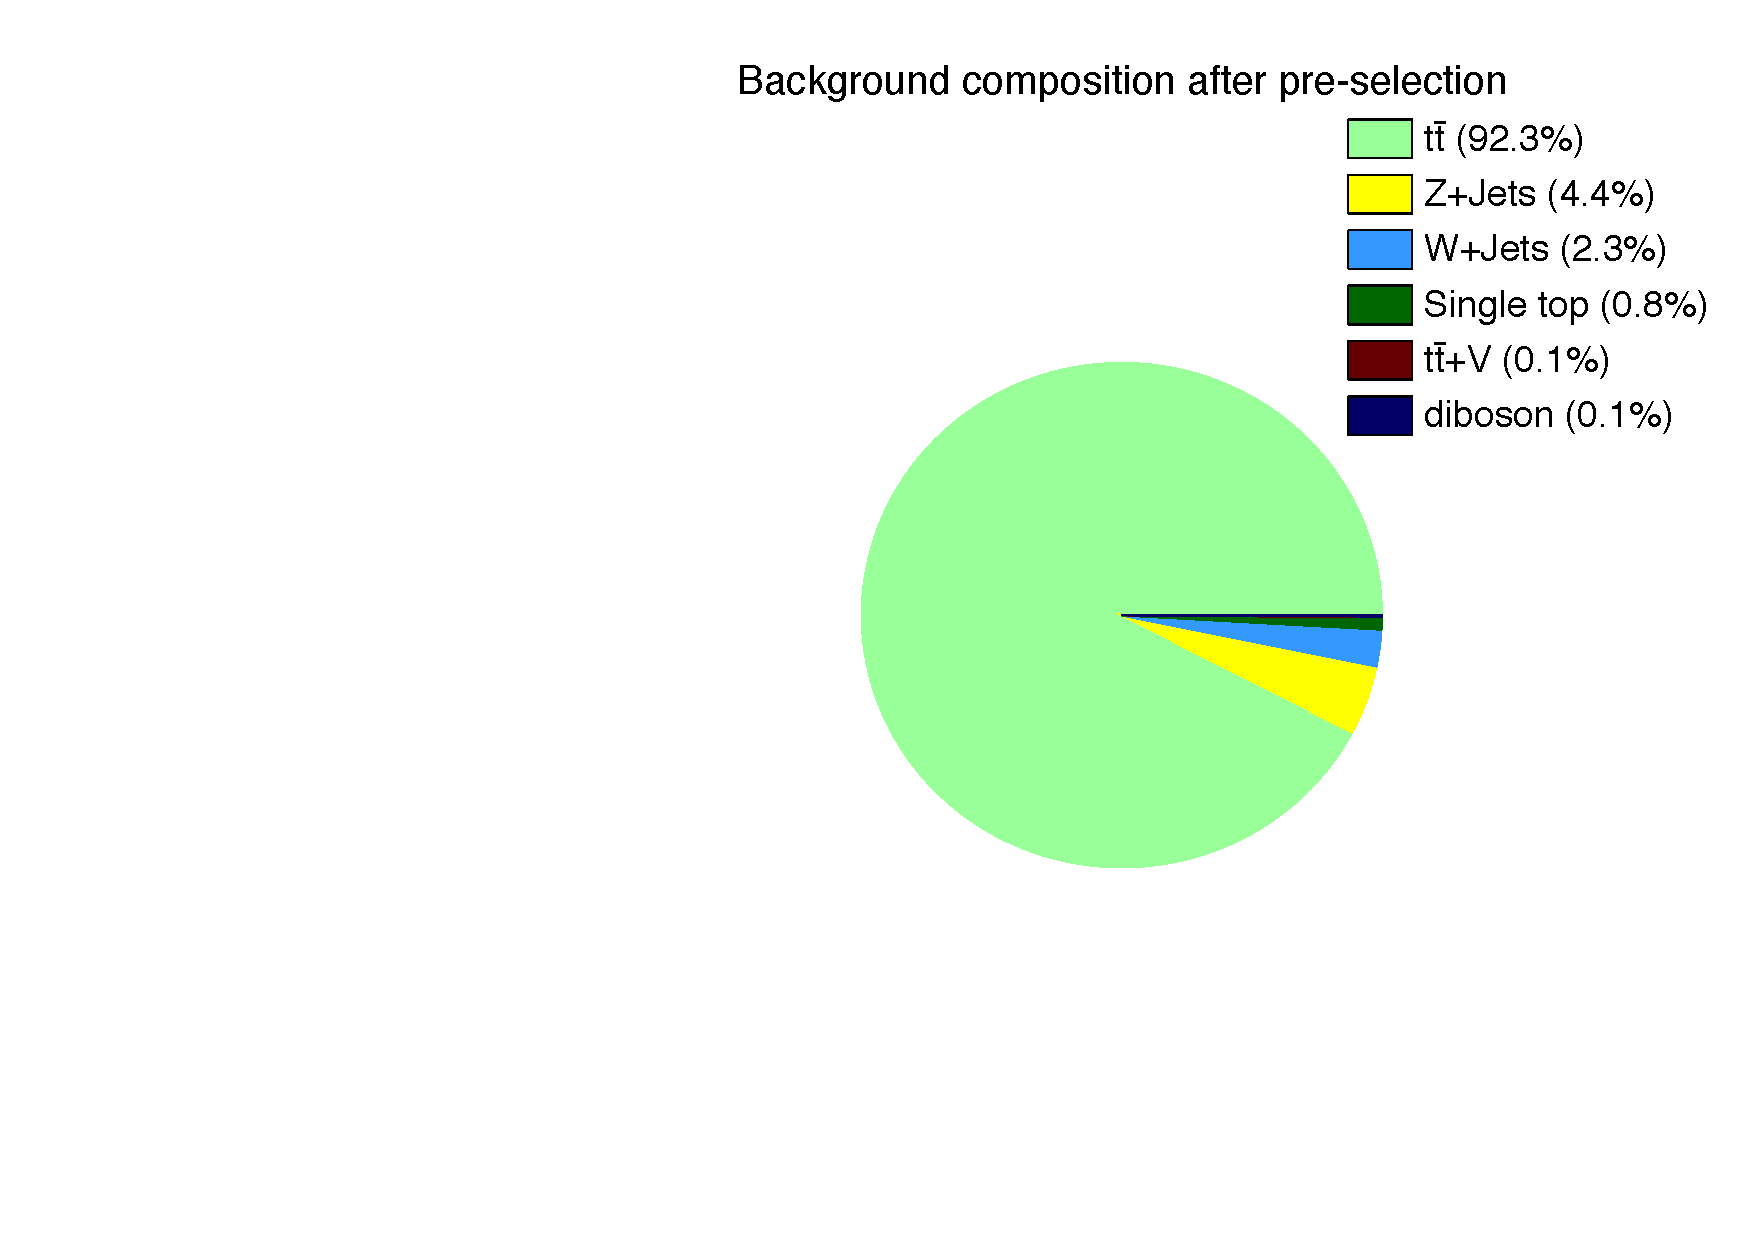
\includegraphics[width=.5\textwidth]{stop/piechart_presel}
				\caption{Pie chart of the background composition after the pre-selection selections described in Table~\ref{tab:SRcommon}}
				\label{fig:piechart_presel}
			\end{wrapfigure}

			Figure~\ref{fig:piechart_presel} displays a pie chart of the \ac{SM} background composition, after having applied all the cuts listed in Table~\ref{tab:SRcommon}. The main background is \ttbar\ production, as a result of the requirement on the number of jets and at least $1$ \bj. The \ttbar\ \ac{MC} sample used here is an inclusive sample\footnote{The sample takes into account all the possible \ttbar\ decays: fully hadronic, semi-leptonic and di-leptonic}.% the semi-leptonic and the di-leptonic \ttbar\ decay would be negligible as a lepton veto is applied.

			The physics objects, reconstructed as discussed in Section~\ref{sec:objReco}, are used to build the various variables used to discriminate the \ac{SUSY} signal from the \ac{SM} background. The event selection is based on such variables which will be described below:

			\begin{description}
				% \item[\boldmath $\htsig$:] An alternate definition of \MET\ significance, where the \sumet\ is replaced by \HT.
				% \item[\boldmath $\meff$:] The effective mass, defined as $\meff = \HT + \met$.
				\item[\boldmath $\mtjetimet$:] The transverse mass (\mt) between the $i^{\mathrm{th}}$ jet and the \met\ in the event. %A massless approximation is used for this and all following \mt\ variables:\newline $\mtjetimet = \sqrt{2\ptjeti\met\left(1-\cos{\Delta\phi\left(\mathrm{jet}^i,\met\right)}\right)}$, where $\ptjeti$ is the transverse momentum of the $i^{\mathrm{th}}$ jet.
				\item[\boldmath $\mtbmin$:] Transverse mass between closest $b$-jet to $\met$ and $\met$. This variable provides very good discrimination between signal and semileptonic \ttbar\ background.
				\item[\boldmath $\mtbmax$:] Transverse mass between farthest $b$-jet to $\met$ and $\met$. This variable provides very good discrimination between signal and semileptonic \ttbar\ background.
				% \item[\boldmath $\mtuntagmetmindphi$:] Transverse mass between closest non-$b$-jet to $\met$ and $\met$. This variable provides  discrimination between signal and EW backgrounds.
				% \item[\boldmath $\mtlowestptmet$:] Transverse mass between the lowest \pt\ \antikt\ $R=0.4$ jets and $\met$. This variable provides extra discrimination between signal and EW backgrounds.
				% \item[\boldmath $\dphibb$:] The azimuthal angle between the two leading $b$-tagged jets in the event. This variable is useful in discriminating against the $Z(\nu\overline\nu)+b\overline{b}+\rm{jets}$ background.
				\item[\boldmath $\drbb$:] The angular separation between the two jets with the highest MV2c10 weight. This variable is useful in discriminating against the $Z(\nu\overline\nu)+b\overline{b}+\mathrm{jets}$ background.
				% \item[\boldmath $m\left(b,b\right)$:] The invariant mass of the two leading $b$-tagged jets in the event. This variable is useful in discriminating against the $Z(\nu\overline\nu)+b\overline{b}+\rm{jets}$ background.
				% \item[\boldmath $\Delta R\left(\bbbar,\textrm{jet}\right)$:] The angular separation between the two leading $b$-tagged jets in the event (presumably from gluon splitting to $\bbbar$ in $Z(\nu\overline\nu)+b\overline{b}+\rm{jets}$) and the closest non $b$-tagged jet.
				% \item[\boldmath $\Delta R\left(\bbbar,\textrm{jet}\right)/\HT$:] The same variable as above, normalized by the \HT.				
			\end{description}


			\paragraph*{Top quark mass reconstruction}

				In addition to the above-mentioned variables, another set of variables is needed in \acp{SR} targeting the pair production of $\stopone \to t + \ninoone$: the reconstruction of two hadronically decaying top quarks in the event using the jet \emph{re-clustering} algorithm, performed using the \antikt\ algorithm (with a larger distance parameter $R = 1.2$), fed with the calibrated \antikt\ $R = 0.4 $jet collection (further details can be found in~\cite{Antikt2008}). The highest- (second-highest) \pt\ re-clustered jet is chosen to be the first (second) top candidate. The best signal sensitivity is reached by using $R = 1.2$ and $R = 0.8$, for top and \Wboson\ candidates, respectively~\cite{stop0L,ICHEPstop0L}. The variables used are the masses of the $R=1.2$ and $R=0.8$ leading and sub-leading jets, indicated by \mantikttwelvezero, \mantikttwelveone, \mantikteightzero, \mantikteightone, respectively. Such variables help reduce the \ac{SM} backgrounds. %from QCD, \Wjets, \Zjets, and lepton + jets \ttbar\ backgrounds,

		\subsection{Optimisation strategy}

		% A crucial step of the cut and count analyses is the optimisation of Signal Regions (SRs) which aim at enhancing the signal yield with respect to the dominant background sources. 
		% Once the events with signal-like properties are identi ed, additional selections are ap- plied to suppress the leftover background whilst retaining the largest possible fraction of signal. This is done using dedicated sets of discriminating variables with di erent dis- tributions in signal and background, that are strongly analysis-dependent and are hence not discussed in the present chapter.

		% The optimisation of SR selections is performed by maximising the value of a  gure of merit (FOM) that represents the discovery signi cance of the signal model of interest (see Section 5.4.2). A variety of de nitions of the signi cance are possible [178], and the analyses in this thesis employ the ZN formula [179], which is implemented in the RooSt- ats package [180] of ROOT [181]. Alternatively, the following simpli ed expression can be used:
		% Nsig
		% Z =  Nbkg + (σbkgNbkg)2 (5.11)
		% where Nsig and Nbkg are the signal and background yields, and σbkg is the an assump- tion on the relative systematic uncertainty on the background. Equation 5.11 is useful to understand intuitively the essential properties of the signi cance, that can be expressed as the ratio of the signal yield in the SR and the total uncertainty on the background, de-  ned as the sum in quadrature of the Poisson error  Nbkg and the expected systematic uncertainty σbkgNbkg.
		% Together with maximising the discovery signi cance, the SR selections must also be chosen depending on the speci c requirements of each search. For example, a given de nition may be preferable because it allows a more robust background estimation, or because it is optimal for a larger number of signal models, or again because it can be combined with other existing channels of the analysis. A tradeo  between these argu- ments and a large value of the signi cance is generally used to converge towards the  nal SR de nition.


	\section{Nominal Background Estimation}
	\label{sec:bkgest}

		\subsection{Control Regions}

		\subsection{Validation Regions}


	\section{Data-Driven Background Estimation}
	\label{sec:ddbkgest}


	\section{Results and Interpretation}
	\label{sec:results}
